%%%%%%%%%%%%%%%%%%%%%%%%%%%%%%%%%%%%%%%%%
% Beamer Presentation
% LaTeX Template
% Version 1.0 (10/11/12)
%
% This template has been downloaded from:
% http://www.LaTeXTemplates.com
%
% License:
% CC BY-NC-SA 3.0 (http://creativecommons.org/licenses/by-nc-sa/3.0/)
%
%%%%%%%%%%%%%%%%%%%%%%%%%%%%%%%%%%%%%%%%%

%----------------------------------------------------------------------------------------
%	PACKAGES AND THEMES
%----------------------------------------------------------------------------------------

\documentclass{beamer}

\mode<presentation> {

% The Beamer class comes with a number of default slide themes
% which change the colors and layouts of slides. Below this is a list
% of all the themes, uncomment each in turn to see what they look like.

%\usetheme{default}
%\usetheme{AnnArbor}
%\usetheme{Antibes}
%\usetheme{Bergen}
%\usetheme{Berkeley}
%\usetheme{Berlin}
%\usetheme{Boadilla}
%\usetheme{CambridgeUS}
%\usetheme{Copenhagen}
%\usetheme{Darmstadt}
%\usetheme{Dresden}
%\usetheme{Frankfurt}
%\usetheme{Goettingen}
%\usetheme{Hannover}
%\usetheme{Ilmenau}
%\usetheme{JuanLesPins}
%\usetheme{Luebeck}
%\usetheme{Madrid}
%\usetheme{Malmoe}
%\usetheme{Marburg}
%\usetheme{Montpellier}
%\usetheme{PaloAlto}
%\usetheme{Pittsburgh}
%\usetheme{Rochester}
%\usetheme{Singapore}
\usetheme{Szeged}
%\usetheme{Warsaw}

% As well as themes, the Beamer class has a number of color themes
% for any slide theme. Uncomment each of these in turn to see how it
% changes the colors of your current slide theme.

%\usecolortheme{albatross}
%\usecolortheme{beaver}
%\usecolortheme{beetle}
%\usecolortheme{crane}
%\usecolortheme{dolphin}
%\usecolortheme{dove}
%\usecolortheme{fly}
%\usecolortheme{lily}
%\usecolortheme{orchid}
%\usecolortheme{rose}
%\usecolortheme{seagull}
%\usecolortheme{seahorse}
%\usecolortheme{whale}
%\usecolortheme{wolverine}
%\usecolortheme{spruce}

%\setbeamertemplate{footline} % To remove the footer line in all slides uncomment this line
%\setbeamertemplate{footline}[page number] % To replace the footer line in all slides with a simple slide count uncomment this line

%\setbeamertemplate{navigation symbols}{} % To remove the navigation symbols from the bottom of all slides uncomment this line
}

\usepackage{graphicx} % Allows including images
\usepackage{booktabs} % Allows the use of \toprule, \midrule and \bottomrule in tables
\usepackage{verbatim}

%----------------------------------------------------------------------------------------
%	TITLE PAGE
%----------------------------------------------------------------------------------------

\title[MASON and ECJ]{MASON and ECJ Integration} % The short title appears at the bottom of every slide, the full title is only on the title page

% This logo will appear on every page.
\logo{%
    
\includegraphics[width=1cm,height=1cm,keepaspectratio]{gmu-logo-1c}~%
    
\includegraphics[width=1cm,height=1cm,keepaspectratio]{nsf-logo}%    
}

\author{AKM Khaled Ahsan Talukder} % Your name
\institute[GMU] % Your institution as it will appear on the bottom of every slide, may be shorthand to save space
{
George Mason University \\ % Your institution for the title page
\medskip
\textit{atalukde@gmu.edu} \\ % Your email address
%\medskip
%\emph{Some portion of this slide is taken from Prof. Sean's talk}
}

%\date{\today} % Date, can be changed to a custom date
\date{June 16, 2013}

\begin{document}

\begin{frame}
\titlepage % Print the title page as the first slide
\end{frame}

%\begin{frame}
%\frametitle{Overview} % Table of contents slide, comment this block out to remove it
%\tableofcontents % Throughout your presentation, if you choose to use \section{} and \subsection{} commands, these will automatically be printed on this slide as an overview of your presentation
%\end{frame}

%----------------------------------------------------------------------------------------
%	PRESENTATION SLIDES
%----------------------------------------------------------------------------------------

%------------------------------------------------
\section{MASON and ECJ}
\begin{frame}
	\frametitle{MASON + ECJ}	
	\begin{block}{}
		\begin{itemize}
			\setlength{\itemsep}{20pt}
			\item MASON: A multiagent simulation toolkit 			
			\item ECJ: A powerful research framework for evolutionary optimzation (which also supports massively parallel optimization)
		\end{itemize}
	\end{block}
	-- both were developed at the Autonomous Robotics Lab, GMU.
\end{frame}
%%
\begin{frame}
	\frametitle{Setting parameters can be a nightmare !}
	\begin{columns}[c]
	\column{2in}
		\centering
		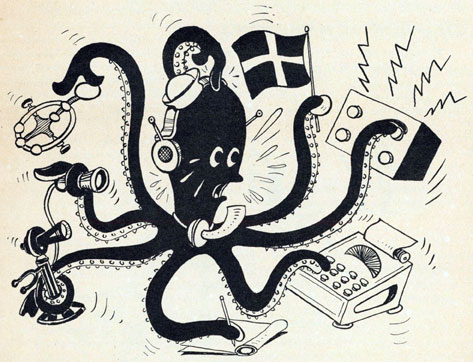
\includegraphics[width=2in,keepaspectratio]{octopus.jpg}
	\column{2.5in}
		%\begin{scriptsize}
			\begin{itemize}
			\setlength{\itemsep}{15pt}
				\item Scientists make \textbf{models}.
				\item Complicated models (i.e. ABM) requires a large number of \textbf{multiple inter-dependent parameters} to be tuned manually -- prohibitive.
				\item \textbf{Can we automate this ?}
			\end{itemize}
		%\end{scriptsize}
	\end{columns}
\end{frame}
%%
\begin{frame}
	\frametitle{Preliminaries}
	\begin{block}{Model Parameter Types}
		\begin{footnotesize}
			\begin{itemize}
				\item Known Parameters -- whose settings already known for a fact
				\item Inferable Parameters -- whose settings should be set in a certain way \\(\emph{according to a particular theory})
				\item Insensitive Parameters -- over whose settings the model is expected to be insensitive
				\item \textbf{Unknown Parameters -- on which an experimenter has no idea/control over.}\\ (\emph{most interesting ?})
			\end{itemize}
		\end{footnotesize}
	\end{block}
	\vspace{-10pt}
	\begin{block}{Goals}
		\begin{footnotesize}
			\begin{itemize}
				\item To produce a certain kind of output which is predicted by a theory, or 
				\item to match and validate against known real-world results.
			\end{itemize}
		\end{footnotesize}
	\end{block}
\end{frame}
%%
\begin{frame}
	\frametitle{Optimization as An Automated Procedure}
	%\begin{columns}[c]
	%\column{3in}
	\vspace{-55pt}
		\begin{figure}
			\centering
			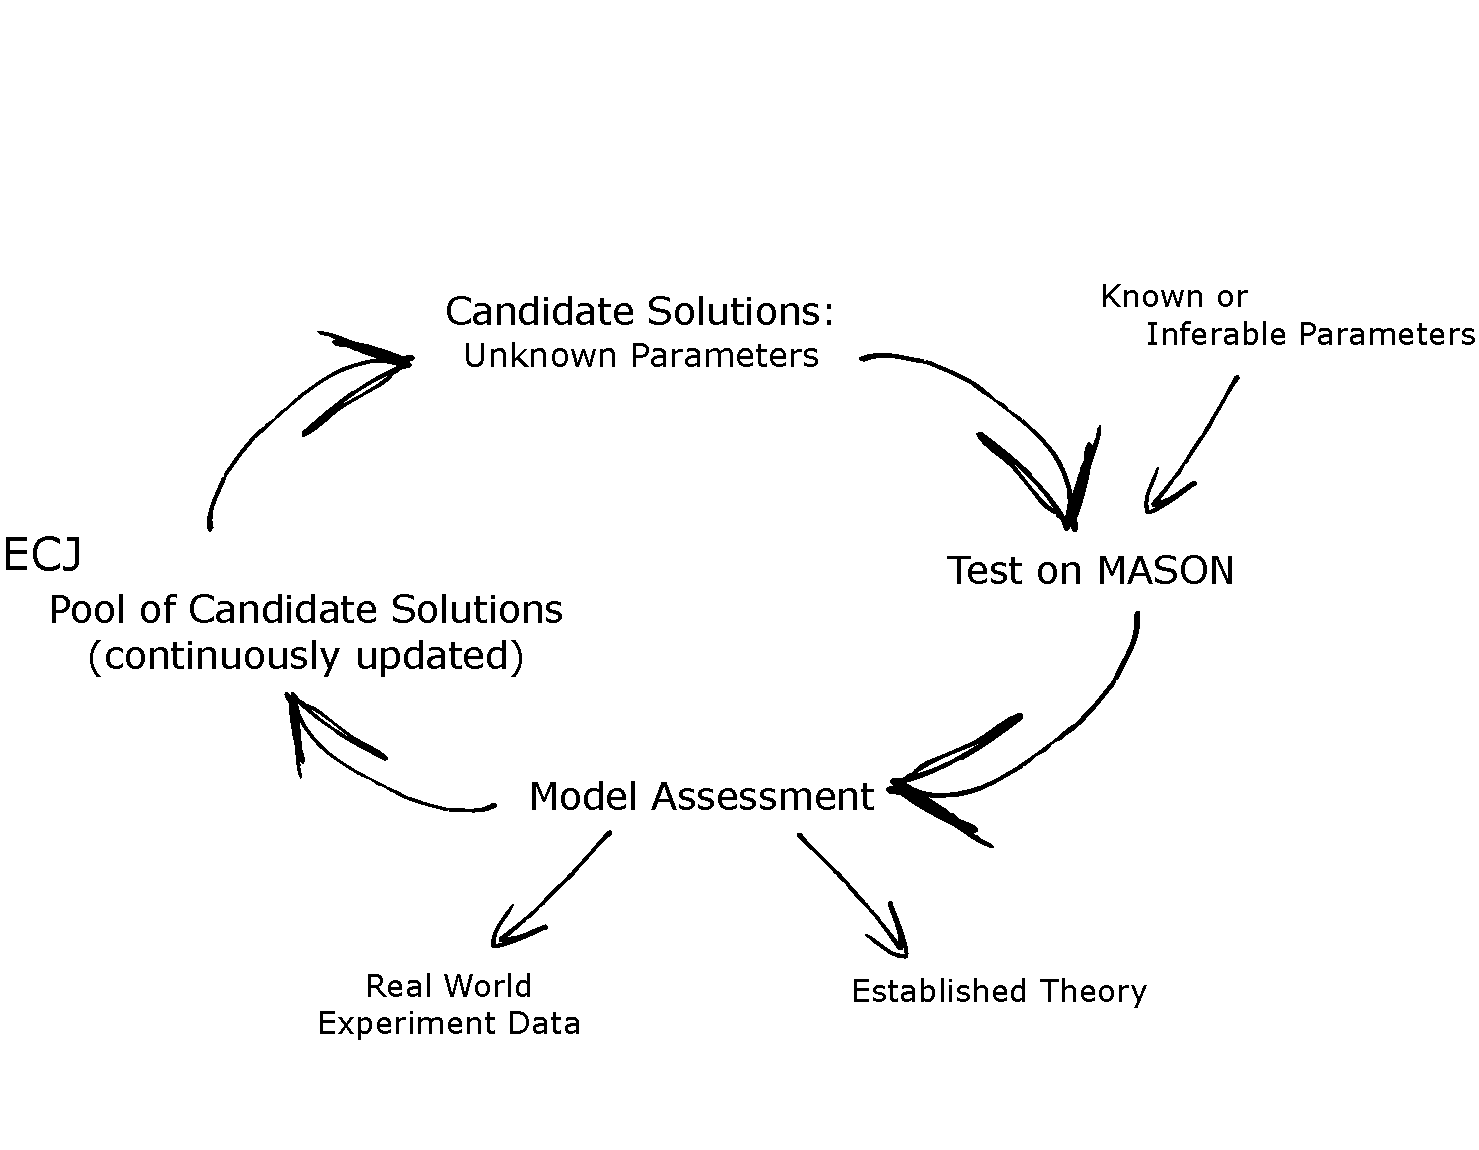
\includegraphics[width=4in,keepaspectratio]{approach-new.pdf}
		\end{figure}
	\vspace{-25pt}
	-- \emph{What if an \textbf{expected} parameter setting is not found ?}
	%\column{2in}
		%\begin{scriptsize}
		%	It's \emph{*still*} interesting even if it fails, since it could reveal -- 
		%	\begin{itemize}
		%		%\setlength{\itemsep}{10pt}
		%		\item \textbf{bug} in the model
		%		\item something \textbf{unforeseen} in the model semantics, or 
		%		\item the theory is \textbf{wrong}
		%	\end{itemize}
		%\end{scriptsize}
	%\end{columns}
\end{frame}
%%
\begin{comment}
\begin{frame}
	\frametitle{Filling The Gap}
	\begin{block}{}
		\centering
		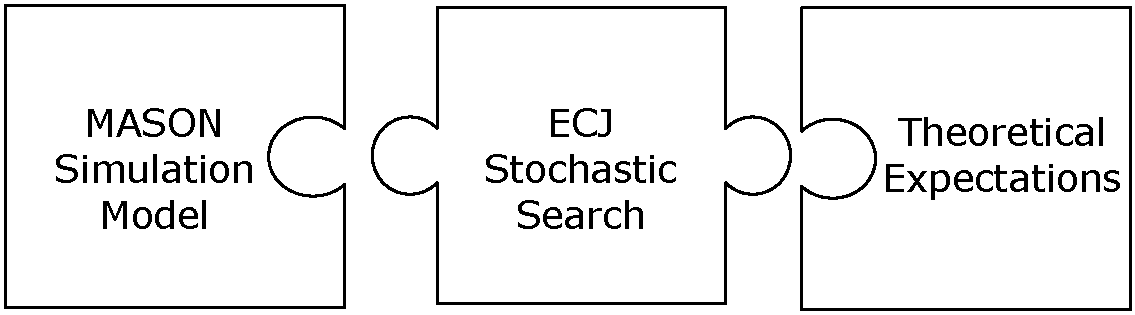
\includegraphics[width=3in,height=2in,keepaspectratio]{gap.pdf}
	\end{block}
\end{frame}
\end{comment}
%%
\begin{frame}
	\frametitle{Parallel Evolutionary Optimization -- A Bird's-Eye View}
	\begin{columns}[c]
	\column{2in}
		%\begin{small}
			\begin{itemize}
			\setlength{\itemsep}{20pt}
				\item Extremely expensive -- need to optimize the model by running it many times.
				\item Ought to be done in parallel.	
			\end{itemize}
		%\end{small}
	\column{3in}
		\centering
		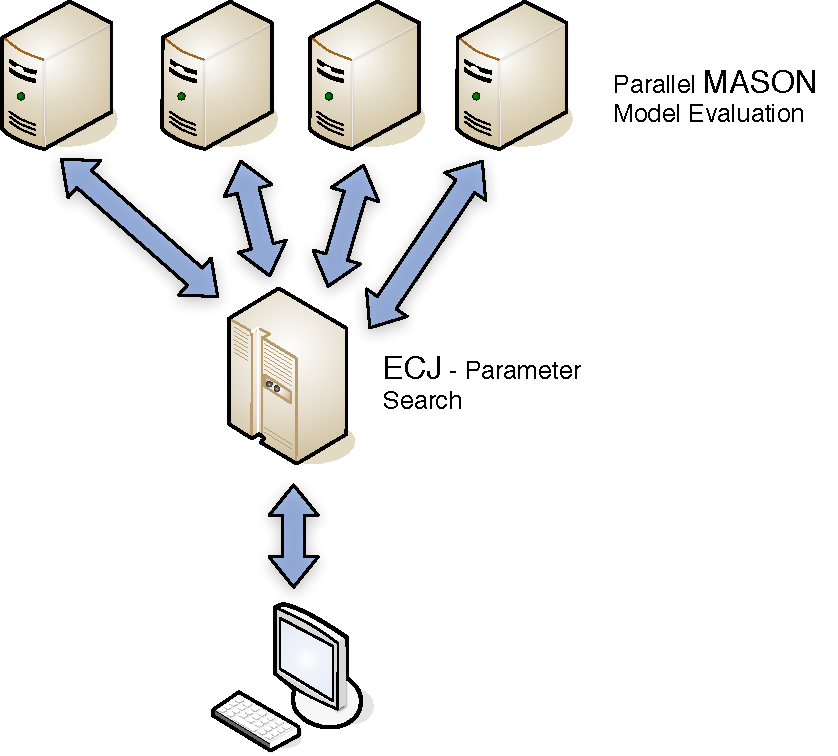
\includegraphics[width=2.5in,keepaspectratio]{master-slave.pdf}	
	\end{columns}
\end{frame}
%------------------------------------------------

%------------------------------------------------
\section{RebeLand}
\begin{frame}	
	\frametitle{First Example -- \textit{RebeLand}}
	\begin{block}{RebeLand -- Simulating a \emph{Society}}
		Model of ``Scoio-Economic Stability'' developed on top of MASON at the Center of Social Complexity, GMU.
	\end{block}
	\begin{block}{Objectives to Maximize (a.k.a \emph{Multi-objective Optimization Problem})}
		\begin{itemize}
			\item Population satisfaction
			\item Amount of money skimmed from the populace through corruption
		\end{itemize}		
	\end{block}
\end{frame}
%%
\begin{frame}
	\frametitle{Parameters/Knobs}
	\begin{block}{Unknown Parameters to Set (\emph{all scaled to 0...1})}
		 \begin{itemize}
			\item State Corruption Rate
			\item State Tax Rate
			\item Maximum State Reserve
			\item Minimum State Reserve
			\item Minimum Spending on Populace
			\item Maximum Police Per Capita
			\item Initial Reserve Army Ratio
			\item Standing Army Size
			\item State Attack Interval
		 \end{itemize}
	\end{block}
\end{frame}
%%
\begin{frame}
	\frametitle{Details You Don't Care About}
	\begin{block}{Optimization Algorithm}
		NSGA-II, 6000 evaluations.
	\end{block}
	\begin{block}{Testing (i.e. \textit{Generalization})}
		Individual \textit{Parameter Settings} are tested by running RebeLand on MASON 8 times -- mean results were considered.
	\end{block}
	\begin{block}{Parallelization}
		Master-Slave Evaluation, 30 Slave Units on Hydra\\
		Total evaluation time: about 1 hour
	\end{block}
\end{frame}
%%
\begin{frame}
	\frametitle{Results: The \emph{Pareto Front}}
	\centering
	\includegraphics[width=2.5in,keepaspectratio,angle=270]{front.eps}
\end{frame}
%%
\begin{frame}
	\frametitle{Results: Population Satisfaction}
	\begin{columns}[c]
	\column{2.5in}
		\centering
		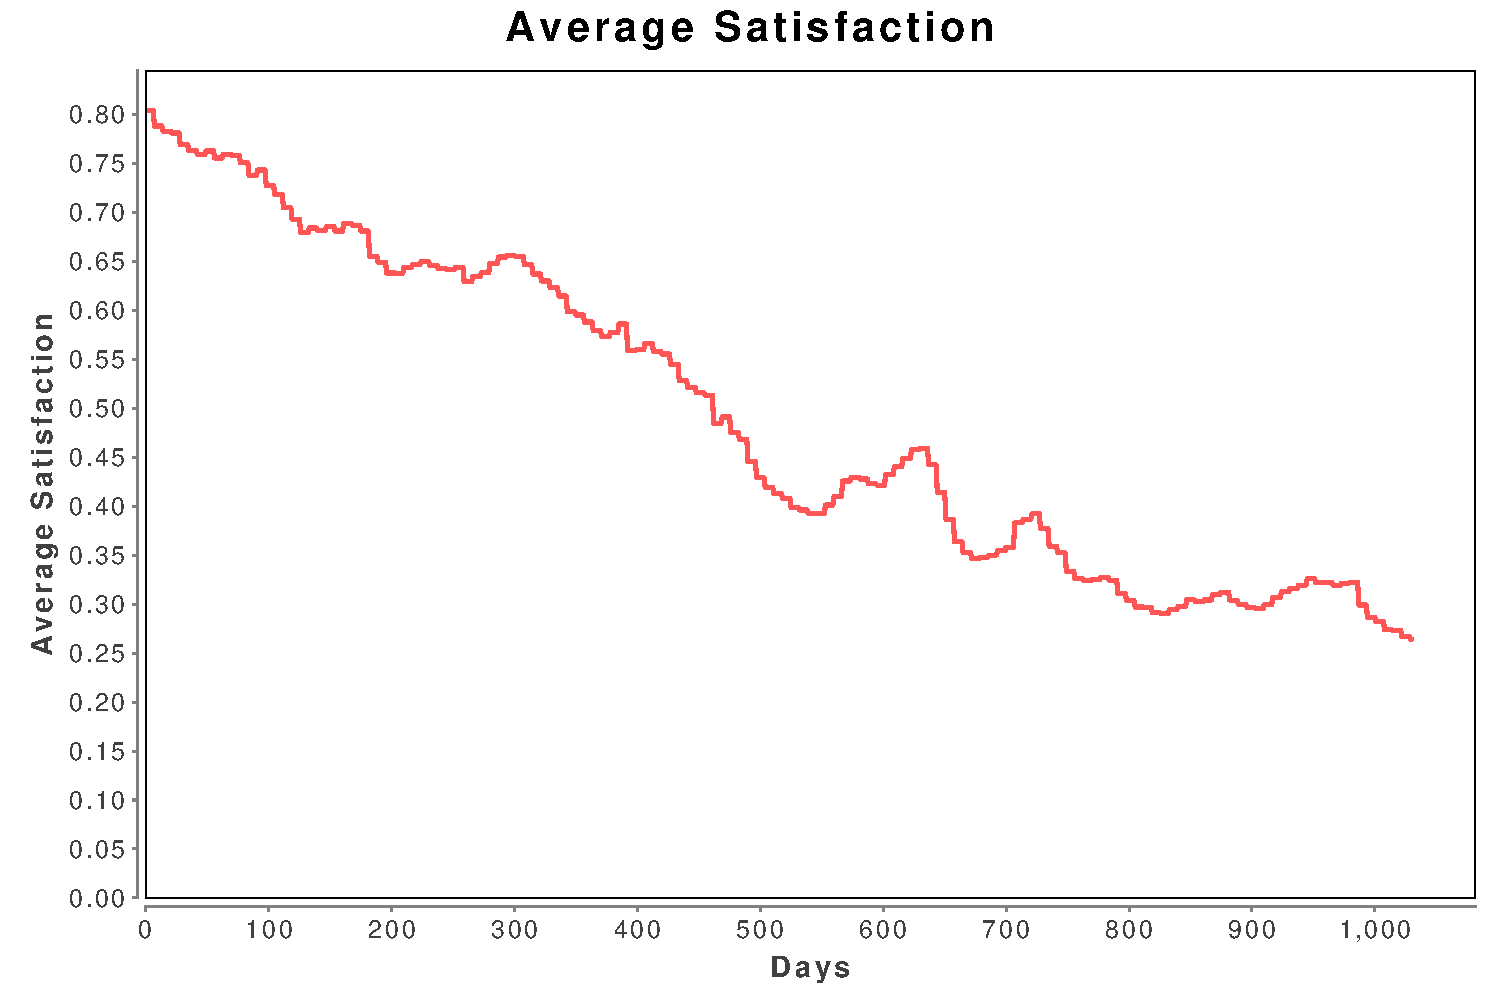
\includegraphics[width=2.25in,keepaspectratio]{average-satisfaction-old.pdf}\\
		Before Optimzation \\(Original Parameters)
	\column{2.5in}
		\centering
		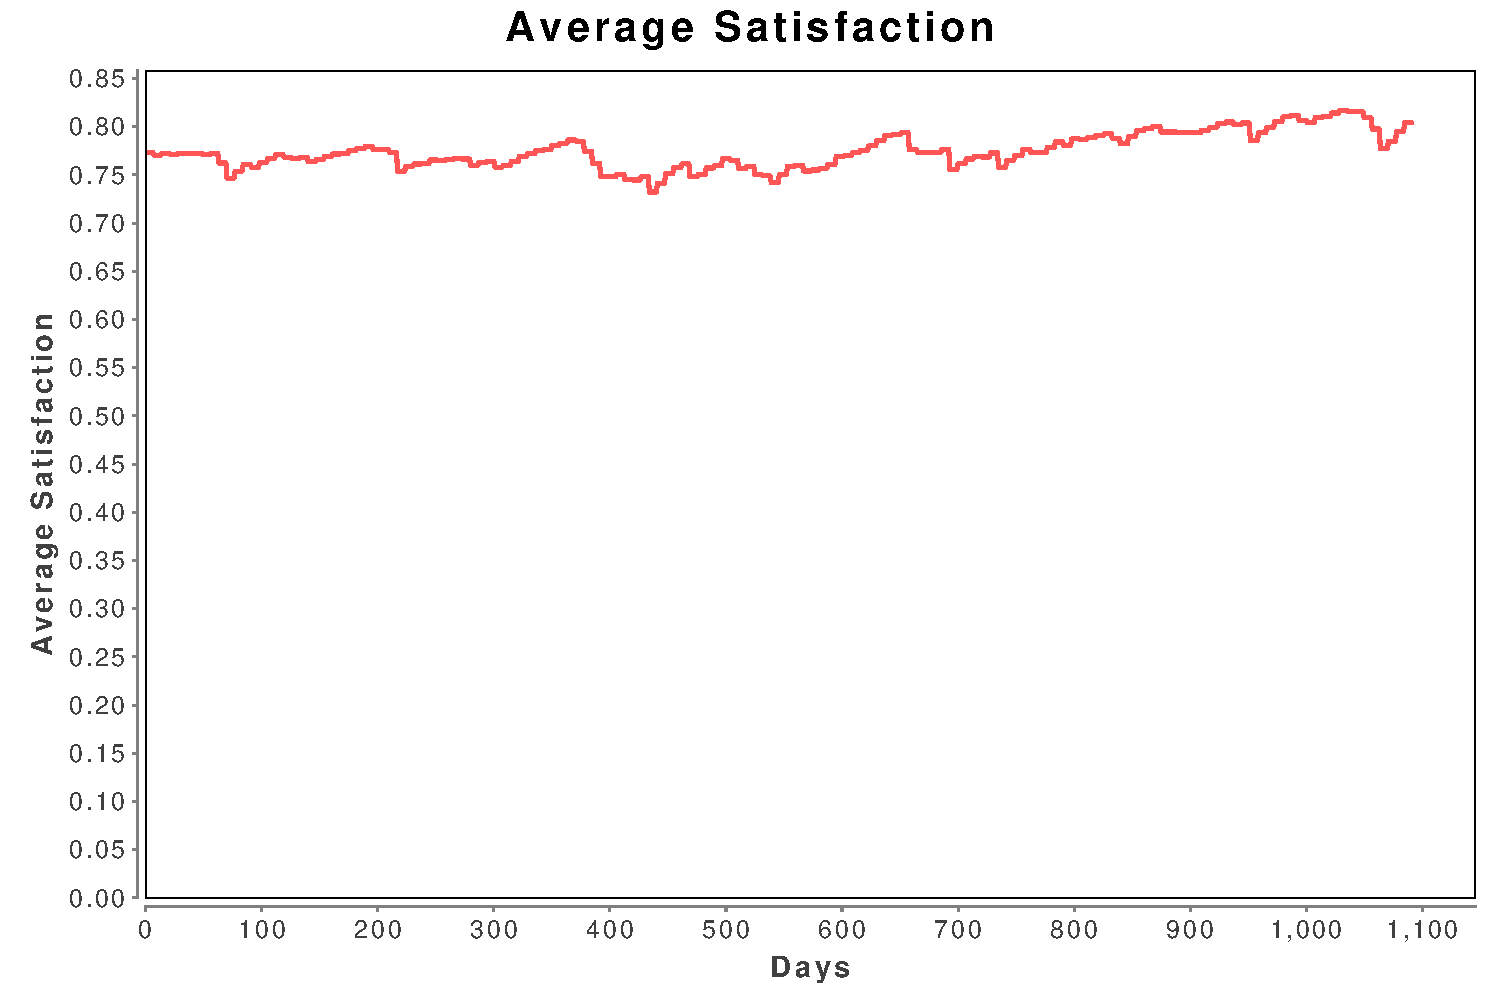
\includegraphics[width=2.25in,keepaspectratio]{average-satisfaction-new.pdf}\\
		After\\ Optimzation
	\end{columns}
\end{frame}
%%
\begin{frame}	
	\frametitle{Results: The Overall Situation}
	\begin{columns}[c]
	\column{2.5in}
		\centering
		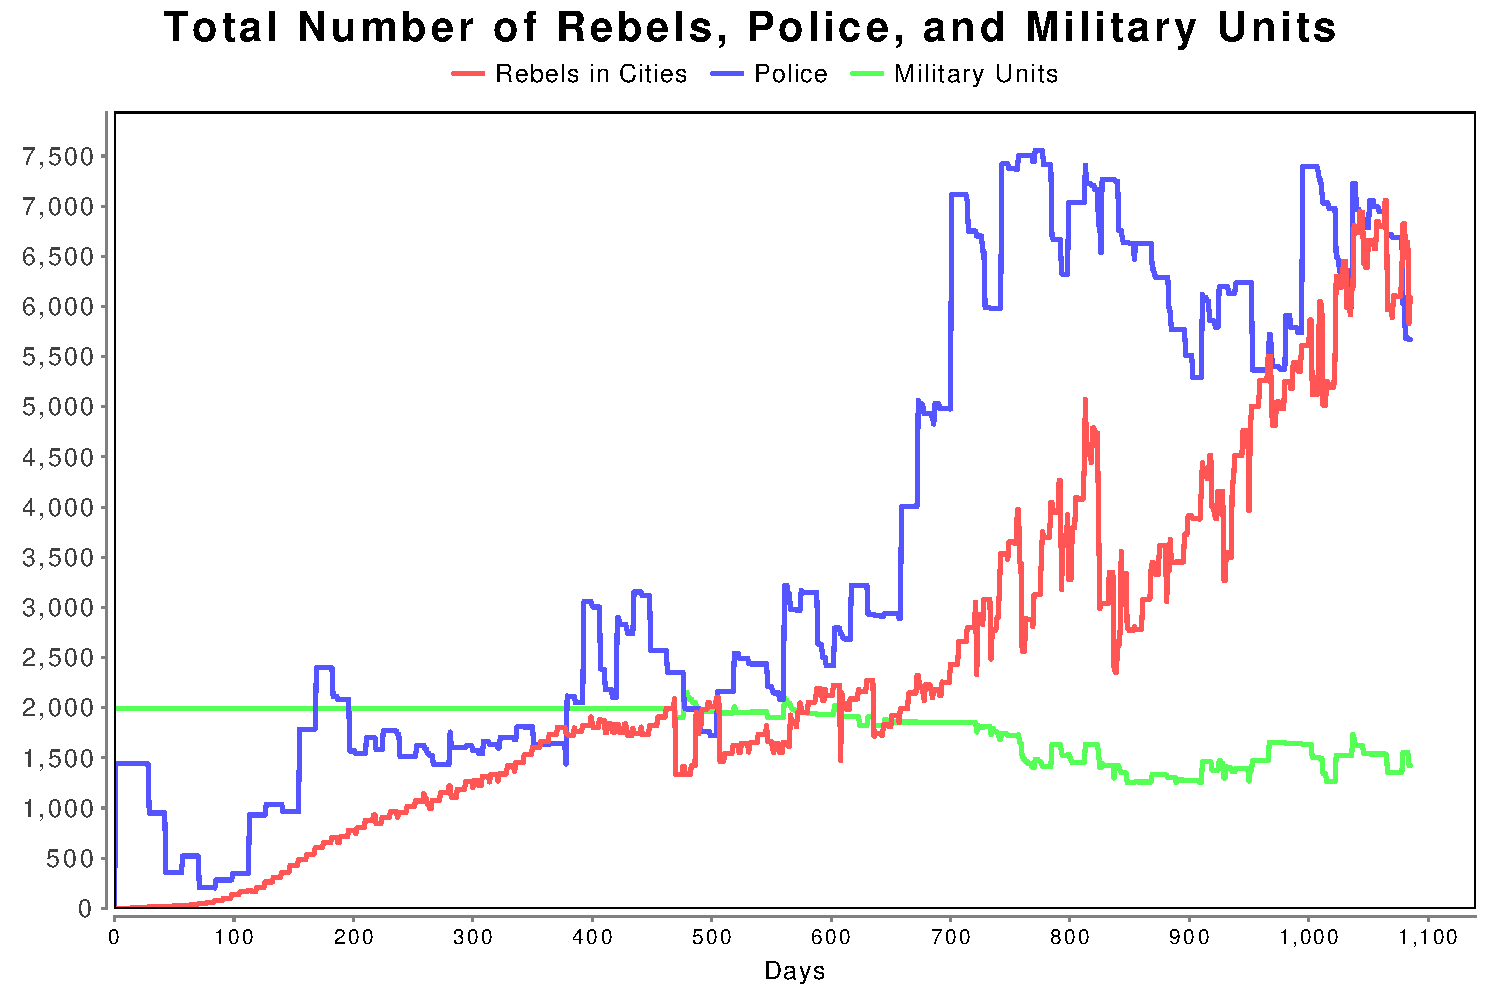
\includegraphics[width=2.25in,keepaspectratio]{situation-old.pdf}\\
		Before Optimzation \\(Original Parameters)
	\column{2.5in}
		\centering
		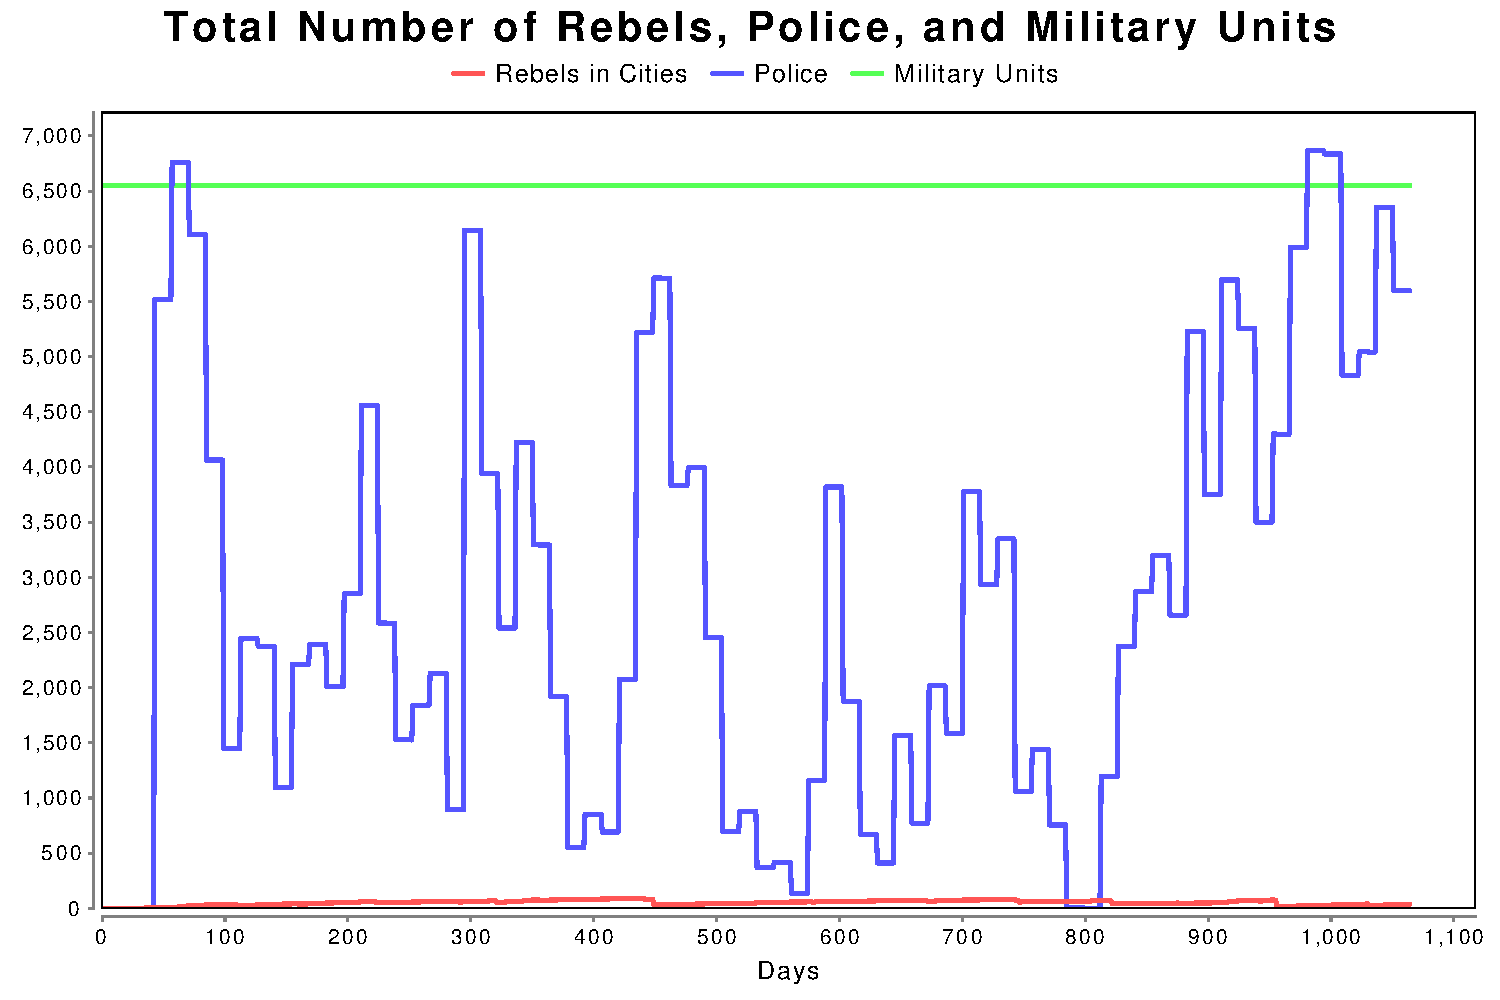
\includegraphics[width=2.25in,keepaspectratio]{situation-new.pdf}\\
		After\\ Optimzation
	\end{columns}
\end{frame}
%%
\begin{frame}
	\frametitle{Results: Some (interesting) numbers}
	\begin{itemize}
		\item State's corruption rate -- \textbf{86\%} 
		\item State's tax rate -- \textbf{77\%}
		\item State's maximum reserve rate -- 84\%
		\item State's minimum reserve rate -- 77\%
		\item Minimum benefit share to the populace (i.e. public spending) -- \textbf{98\%}
		\item Maximum number of police force per capita -- \textbf{31\%}
		\item Initial reserve army ratio -- 0.01\%
		\item Standing army size -- 0.06\%
		\item State's attack frequency (to suppress rebels) -- \textbf{78\%}
	\end{itemize}
\end{frame}
%%
\begin{frame}
	\frametitle{Conclusions}
	\begin{block}{Lesson ?}
		It's \textbf{fine} to run a \textbf{corrupt} government and keep its people \textbf{happy} -- \emph{only} if you have a \textbf{high} public spending, \textbf{large police force} and a very \textbf{frequent attack} on rebels.
	\end{block}
	\begin{block}{Utopia ?}
		These results are ``interesting'' -- i.e. \textit{communist dictatorship} ?
	\end{block}
	\begin{block}{Revelations ?}
		Does this reveal cracks in the \emph{RebeLand} model semantics? Or a bug in the code?
	\end{block}
\end{frame}
%------------------------------------------------

%------------------------------------------------
\section{PacMan}
\begin{frame}
	\frametitle{Next: PacMan -- Evolving Agent Behaviour}
	\begin{block}{}
		\begin{itemize}
			\setlength{\itemsep}{0.75cm}
			\item MASON $\rightarrow$ \textbf{Behaviour} specifications
			\item ECJ $\rightarrow$ \textbf{Optimization} by \textbf{Evolution}
			\item MASON $+$ ECJ $\rightarrow$ Evolving Optimized Behaviour
			\item \textbf{Target}: The game of PacMan 
		\end{itemize}
	\end{block}
\end{frame}
%%
\begin{comment}
	\begin{frame}
		\frametitle{A Slight Digression}
			We tried to implement this framework by keeping these key design goals in mind -- \\
			\begin{itemize}
				\setlength{\itemsep}{0.5cm}
				\item Reuse the codes in the existing MASON models extensively.
				\item Apply all necessary MASON model specifications in ECJ parameter files.
				\item In some cases, \emph{Java Reflections} could be a better way to achieve.
			\end{itemize}
	\end{frame}
%%
\begin{frame}
	\frametitle{Some Technical Information}
	\begin{footnotesize}
	\begin{block}{Optimization Algorithm}
		Koza Style \emph{Genetic Programming}, 6000 evaluations ($=$ 60 individuals $\times$ 100 Generations). Distributed evolution is also possible.
	\end{block}
	\begin{block}{Genetic Programming}
		Agent's behaviour is encoded as a \textbf{tree} of basic maneuvers. Start with a \textbf{set of randomly generated trees}, use \textbf{breeding mechanism} to \textbf{evolve} them into an \textbf{optimized} behaviour for an agent to \textbf{win a game}, in our case, a PacMan game.
	\end{block}	
	\begin{block}{Objective Function}
		A ``better'' behaviour $\leftarrow$ $f(\text{game score}, \ldots)$
	\end{block}
	\end{footnotesize}
\end{frame}
\end{comment}
%%
\begin{frame}
	\frametitle{An Evolved Pac Behaviour}
	\begin{block}{}
		\centering
		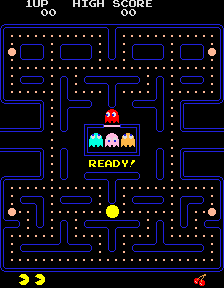
\includegraphics[width=1.5in,keepaspectratio]{pac-man.png}
	\end{block}
	\vspace{-25pt}
	\begin{block}{}
		\Huge{\centerline{Demo}}
	\end{block}
\end{frame}
%------------------------------------------------

%------------------------------------------------
\section{Summary}
\begin{frame}
	\frametitle{Summary}
	\begin{columns}[c]
		\column{2.5in}
			\centering
			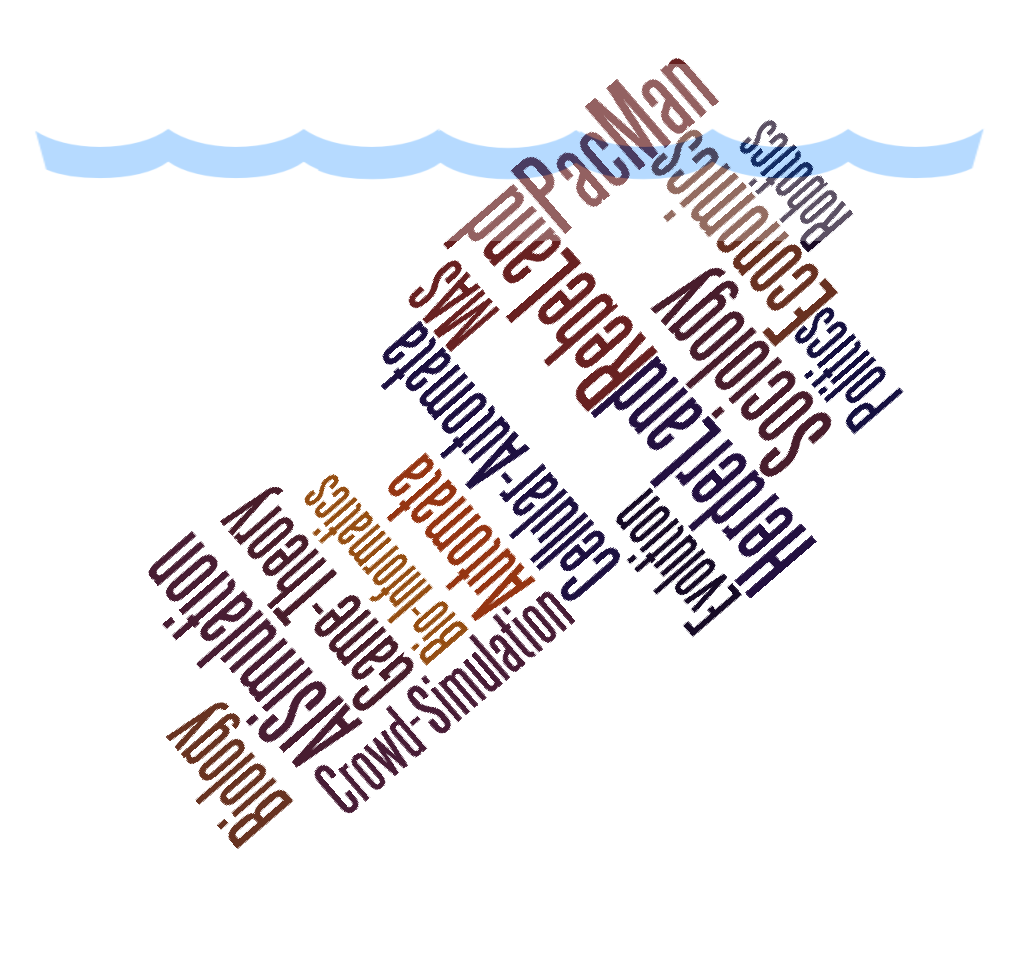
\includegraphics[width=2.5in,keepaspectratio]{iceberg.pdf}
		\column{2in}
		\begin{footnotesize}
			\begin{itemize}
				\setlength{\itemsep}{0.30cm}
				\item Parameter optimization could be very important for assessing a \textbf{model's validity}, finding \textbf{more interesting insights}.
				\item Surely, symbiosis between MASON and ECJ -- has a lot more to offer.
				\item Building a unified/standardized APIs to help plugging ECJ capabilities into MASON models -- could just be a tip of the iceberg.
			\end{itemize}
		\end{footnotesize}
	\end{columns}
\end{frame} 
%------------------------------------------------

%------------------------------------------------
\section{Feedback}
	\begin{frame}
		\begin{block}{}
			\Huge{\centerline{Questions?}}
		\end{block}
		\begin{block}{}
			\Huge{\centerline{Suggestions?}}
		\end{block}
	\end{frame}
%------------------------------------------------

\begin{comment}
%------------------------------------------------
\section{First Section} % Sections can be created in order to organize your presentation into discrete blocks, all sections and subsections are automatically printed in the table of contents as an overview of the talk
%------------------------------------------------

\subsection{Subsection Example} % A subsection can be created just before a set of slides with a common theme to further break down your presentation into chunks

\begin{frame}
\frametitle{Paragraphs of Text}
Sed iaculis dapibus gravida. Morbi sed tortor erat, nec interdum arcu. Sed id lorem lectus. Quisque viverra augue id sem ornare non aliquam nibh tristique. Aenean in ligula nisl. Nulla sed tellus ipsum. Donec vestibulum ligula non lorem vulputate fermentum accumsan neque mollis.\\~\\

Sed diam enim, sagittis nec condimentum sit amet, ullamcorper sit amet libero. Aliquam vel dui orci, a porta odio. Nullam id suscipit ipsum. Aenean lobortis commodo sem, ut commodo leo gravida vitae. Pellentesque vehicula ante iaculis arcu pretium rutrum eget sit amet purus. Integer ornare nulla quis neque ultrices lobortis. Vestibulum ultrices tincidunt libero, quis commodo erat ullamcorper id.
\end{frame}

%------------------------------------------------

\begin{frame}
\frametitle{Bullet Points}
\begin{itemize}
\item Lorem ipsum dolor sit amet, consectetur adipiscing elit
\item Aliquam blandit faucibus nisi, sit amet dapibus enim tempus eu
\item Nulla commodo, erat quis gravida posuere, elit lacus lobortis est, quis porttitor odio mauris at libero
\item Nam cursus est eget velit posuere pellentesque
\item Vestibulum faucibus velit a augue condimentum quis convallis nulla gravida
\end{itemize}
\end{frame}

%------------------------------------------------

\begin{frame}
\frametitle{Blocks of Highlighted Text}
\begin{block}{Block 1}
Lorem ipsum dolor sit amet, consectetur adipiscing elit. Integer lectus nisl, ultricies in feugiat rutrum, porttitor sit amet augue. Aliquam ut tortor mauris. Sed volutpat ante purus, quis accumsan dolor.
\end{block}

\begin{block}{Block 2}
Pellentesque sed tellus purus. Class aptent taciti sociosqu ad litora torquent per conubia nostra, per inceptos himenaeos. Vestibulum quis magna at risus dictum tempor eu vitae velit.
\end{block}

\begin{block}{Block 3}
Suspendisse tincidunt sagittis gravida. Curabitur condimentum, enim sed venenatis rutrum, ipsum neque consectetur orci, sed blandit justo nisi ac lacus.
\end{block}
\end{frame}

%------------------------------------------------

\begin{frame}
\frametitle{Multiple Columns}
\begin{columns}[c] % The "c" option specifies centered vertical alignment while the "t" option is used for top vertical alignment

\column{.45\textwidth} % Left column and width
\textbf{Heading}
\begin{enumerate}
\item Statement
\item Explanation
\item Example
\end{enumerate}

\column{.5\textwidth} % Right column and width
Lorem ipsum dolor sit amet, consectetur adipiscing elit. Integer lectus nisl, ultricies in feugiat rutrum, porttitor sit amet augue. Aliquam ut tortor mauris. Sed volutpat ante purus, quis accumsan dolor.

\end{columns}
\end{frame}

%------------------------------------------------
\section{Second Section}
%------------------------------------------------

\begin{frame}
\frametitle{Table}
\begin{table}
\begin{tabular}{l l l}
\toprule
\textbf{Treatments} & \textbf{Response 1} & \textbf{Response 2}\\
\midrule
Treatment 1 & 0.0003262 & 0.562 \\
Treatment 2 & 0.0015681 & 0.910 \\
Treatment 3 & 0.0009271 & 0.296 \\
\bottomrule
\end{tabular}
\caption{Table caption}
\end{table}
\end{frame}

%------------------------------------------------

\begin{frame}
\frametitle{Theorem}
\begin{theorem}[Mass--energy equivalence]
$E = mc^2$
\end{theorem}
\end{frame}

%------------------------------------------------

\begin{frame}[fragile] % Need to use the fragile option when verbatim is used in the slide
\frametitle{Verbatim}
\begin{example}[Theorem Slide Code]
\begin{verbatim}
\begin{frame}
\frametitle{Theorem}
\begin{theorem}[Mass--energy equivalence]
$E = mc^2$
\end{theorem}
\end{frame}\end{verbatim}
\end{example}
\end{frame}

%------------------------------------------------

\begin{frame}
\frametitle{Figure}
Uncomment the code on this slide to include your own image from the same directory as the template .TeX file.
%\begin{figure}
%\includegraphics[width=0.8\linewidth]{test}
%\end{figure}
\end{frame}

%------------------------------------------------

\begin{frame}[fragile] % Need to use the fragile option when verbatim is used in the slide
\frametitle{Citation}
An example of the \verb|\cite| command to cite within the presentation:\\~

This statement requires citation \cite{p1}.
\end{frame}

%------------------------------------------------

\begin{frame}
\frametitle{References}
\footnotesize{
\begin{thebibliography}{99} % Beamer does not support BibTeX so references must be inserted manually as below
\bibitem[Smith, 2012]{p1} John Smith (2012)
\newblock Title of the publication
\newblock \emph{Journal Name} 12(3), 45 -- 678.
\end{thebibliography}
}
\end{frame}

%------------------------------------------------

\begin{frame}
\Huge{\centerline{The End}}
\end{frame}
%----------------------------------------------------------------------------------------
\end{comment}

\end{document} 
